The CMB monopole signal, or equivalently its average intensity across the sky, was first observed in New Jersey (see Section~\ref{sec:cmb}) as a faint buzz at a frequency of 5~GHz that was constant in time, space, and intensity. This signal turned out to have a blackbody spectrum with a temperature of $T_{\mathrm{CMB}} = 2.7$~K. As discussed in Section~\ref{sec:anisotropies}, CMB temperature anisotropies are $\sim$~1/10,000 time smaller than the monopole, and therefore Penzias and Wilson's intensity measurement appeared to be constant with sky location

The Simons Array (SA) is a CMB observatory located on Cerro Toco in the Atacama Desert of Chile at an elevation of 5,200~m. It aims to achieve state-of-the-art large-angular-scale sensitivity using multi-chroic, large-aperture telescopes, simultaneously enabling delensing and galactic foreground subtraction in the hunt for primordial B-modes. SA consists of three telescopes in total, each housing a dichroic POLARBEAR-2 (PB-2) receiver cryostat: PB-2a and PB-2b observe at 90 and 150~GHz, while PB-2c observes at 220 and 270~GHz. Each telescope has a 2.5~m primary mirror in an off-axis Gregorian configuration\cite{tran_comparison_2008} and generates 5.2, 3.5, 2.7, and 2.2 arcmin beams at 90, 150, 220, and 270~GHz, respectively.  Each receiver cryostat has a 0.5~m vacuum window aperture, three 4~K alumina reimaging lenses, a 4~K Lyot stop, and a 365~mm diameter, 0.3~K focal plane of 7,588 transition-edge sensor (TES) bolometers. PB-2a achieved first light in January 2019,\cite{kaneko_deployment_2020} PB-2b\cite{howe_design_2018} is deployed to Chile, and PB-2c is under development.

In order to improve the image quality over a larger field of view, the telescope image is said to be ``reimaged'' by the \texit{receiver cryostat} (which is also often referred to as the \textit{camera}). 

Because each SA receiver observes in two bands, the AR coating needs to be braodband, and PB-2a/b/c achieve this by using coatings with multiple layers of optimal index and cut to optimal thickness.

\begin{figure}
    \centering
    \includegraphics[width=0.95\linewidth]{POLARBEAR-2/Figures/PB2_telescope.jpg}
    \caption[POLARBEAR-2 telescope]{Photograph of the POLARBEAR-2 telescope. The primary and secondary mirros for an off-axis Gregorian pair. The primary reflector has a diameter of 3 m, which provides arcminute-scale angular resolution, but the compact design allows for relatively easy telescope motion. This unique combination of a large reflector and compact telescope provides POLARBEAR-2 with observational versatiliy.}
    \label{fig:pb2_telescope}
\end{figure}

\footenote{The South Pole does have its advantages, though, including better weather stability, as the sun rises and sets only once per year.}

As mentioned above, water in the atmosphere attenuates the CMB signal while also generating parasitic thermal emission. 

\begin{figure}
    \centering
    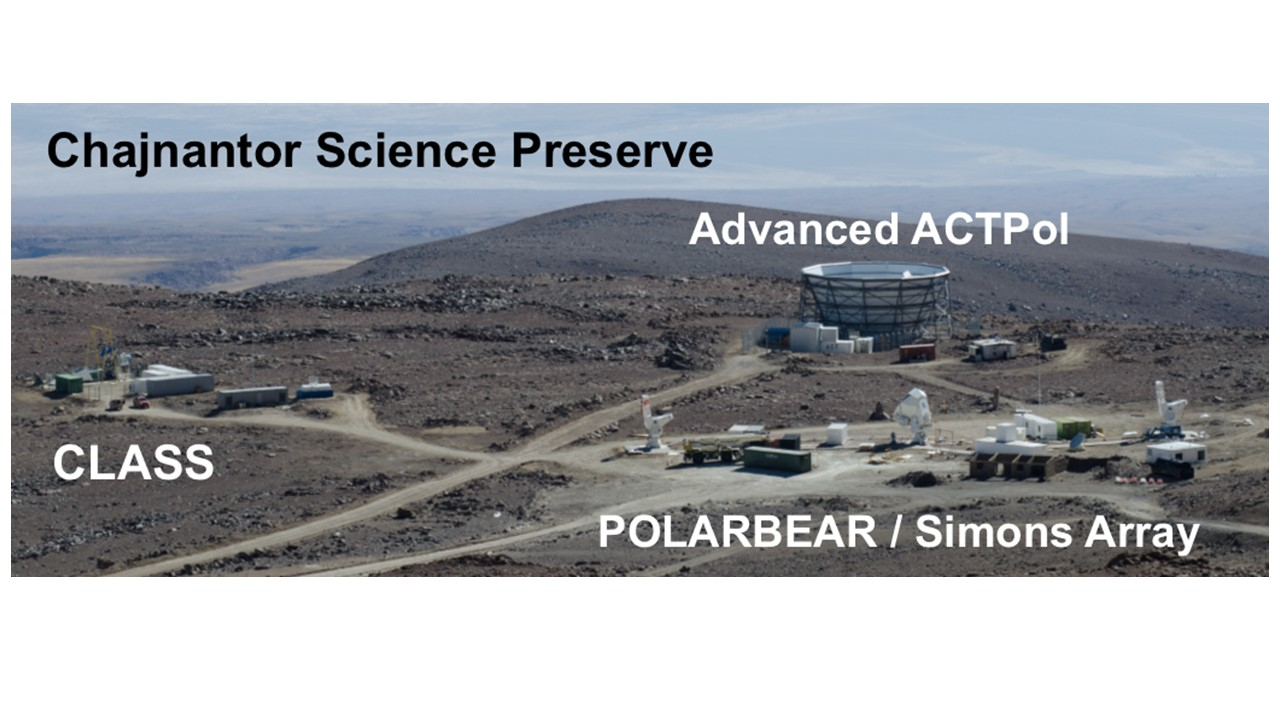
\includegraphics[width=\linewidth, trim=0cm 4cm 0cm 4cm clip]{POLARBEAR-2/Figures/chajnantor_site.jpg}
    \caption[Chajnantor observation site]{Photograph of the observation site for Simons Array. Three PB2-style telescopes operate at 5,200 m elevation and neighbor Advanced ACT, CLASS, and Simons Observatory. PB2b operates on the southernmost of these three telescopes, which is furthest to the left. Figure courtesy of Nathan Stebor.}
    \label{fig:chajnantor_site}
\end{figure}

As mentioned earlier in Section~\ref{sec:simons_array}, SA consists of three identical telescopes, each housing a distinct cryogenic receiver: PB-2a, PB-2b, and PB-2c. In this section, we discuss the specifics of the SA optical systems. 

Adding to the discussion of the Lyot stop, another critically important function of the receiver cryostat is to couple the sky image to the detector efficiently. The quality of the coupling is, in the diffraction-limited regime, determined by the F-number at the focal plane. As shown in Equation~blah, the angular beam profile of the detector pixel depends on its diameter. In addition, the magnification of the camera is governed by its magnification. 

The larger the pixel, the larger the Lyot stop spillover efficiency, or equivalently the less of the detector pixel's beam is dumped onto the stop. In this way, a larger pixel is said to better couple to the telescope, while a smaller pixel will, in the reverse-time-sense, dump more power onto the stop, and hence be more efficient. 

Equation~\ref{eq:beam_coupling_efficiency} is a major component of the focal plane layout optimization. The SA and SO receivers are FOV-limited and therefore have a fixed focal plane area with acceptable image quality. Assuming a readout scheme with functionally limitless capacity, there is a trade off of sensitivity vs pixel size: smaller pixels allow for a larger pixel density, which in the presence of a fixed focal plane area allows for more pixels, while larger pixels provide better sensitivity per pixel. These competing effects combine to give peak in instrument sensitivity vs pixel diameter. We discuss pixel density optimization in great detail in Section~blah, but the chosen pixel diameters for SA and SO along with their beam coupling efficiencies are given in Table~\ref{tab:beam_coupling_efficiencies}.

Because the primary mirror has a finite extent, a major function of the receiver cryostat is to limit the illumination of the primary mirror., which is achieved via the Lyot stop. the illumination pattern of detector pixels onto the primary mirror (in the reverse-time sense) can spill over the mirror edges, which in turn can add large amounts of 300~K radiation from the ground and surroundings into the optical system. A Lyot stop's function is to limit the illumination of the primary mirror by truncating angular response of the detectors on the focal plane onto a cold surface. While this truncation induces diffraction, and also limits the angular resolution of the instrument on the sky, it ensures that the primary mirror is not over-illuminated, replacing what would be 300~K spillover with 4~K spillover, which in turn dramatically mm-wave emission onto the detectors. Additionally, controlling spill to 300~K will limit ground pickup, which is important for suppressing scan-synchronous signals.

As shown in Figure~\ref{fig:bolo_operation}, the bolometer's operating resistance is $R_{\mathrm{bolo}} \approx 1$~$\Omega$, and if parasitic impedances are of the same order, $\delta P_{\mathrm{bias}} / \delta P_{\mathrm{opt}}$ will fall and responsivity will suffer. In addition, because each bolometer is biased with a different frequency and because parasitic impedances are in general frequency-dependent, changes in responsivity across a given comb and across the focal plane are common. As a result, bolometer + readout characterization is central to a successful calibration of sky power to amplifier output. This reality is in contrast to time-domain multiplexing, which DC biases bolometers and therefore does not need to worry about cable inductances and connector capacitances at high frequencies.

Modern day readout techniques allow thousands of detectors be read out from the focal plane, allowing for modest per-detector beam coupling efficiencies in favor of higher pixel densities, which together improve overall instrument sensitivity.